\documentclass[12pt,a4paper]{article}

% Paquetes de configuración del documento
\usepackage[utf8]{inputenc}
\usepackage[spanish]{babel}
\usepackage[T1]{fontenc}
\usepackage[margin=2.5cm]{geometry}
\usepackage{fancyhdr}
%Paquetes para simbologia%
\usepackage{amsmath}
\usepackage{amsfonts}
\usepackage{amssymb}
\usepackage{physics}
\usepackage{longtable}
\usepackage{graphicx}
\usepackage{caption}
\usepackage{float}
\usepackage[hyphens]{url}        % Permite cortar URLs largas con guiones
\usepackage[colorlinks=true,
            linkcolor=black,
            urlcolor=myblue,
            citecolor=black,
            filecolor=black]{hyperref}
 % Opción estándar para enlaces
\Urlmuskip=0mu plus 1mu          % Mejora el espaciado para permitir cortes
\usepackage{subcaption}  % en el preámbulo
\usepackage{pgfplots}
\pgfplotsset{compat=1.18}
\usepackage{tikz}
\usepackage{xcolor}
\definecolor{myblue}{RGB}{42, 127, 179}

\pagestyle{fancy}
\chead{\textit{Materiales Metálicos}}
\rhead{\textit{UTN-FRVM}}
\lhead{\textit{Ingeniería Mecánica}}

\begin{document}
\begin{titlepage}
	
	\begin{center}
		{\huge \textit{Universidad Tecnológica Nacional}}\\
        \vspace{0.5cm}
		{\LARGE \textit{Facultad Regional Villa María}}\\
		\vspace{1.5cm}
        {\LARGE{\textit{Ingeniería Mecánica - Materiales Metálicos}}}\\
		\vspace{1.5cm}
        \LARGE{\textit{Trabajo Práctico 3-06}}
	\end{center}
	
	\vfill

    \textit{Grupo DEL RÍO:}
	\begin{itemize}
		\item \textit{Abregú, Iván.}
		\item \textit{Antico, Rodrigo.}
		\item \textit{Brussa,Julián.}
		\item \textit{Cabral, Franco.}
        \item \textit{Cárdenas, Felipe.}
        \item \textit{Cardozo, Martín.}
        \item \textit{Córdoba, Nathan.}
        \item \textit{Cucco, Ramiro.}
        \item \textit{del Río, Juan.}
        \item \textit{Guerini, Nazareno.}
        \item \textit{Medina, Ivo.}
        \item \textit{Ortiz, Gastón.}
        \item \textit{Picos, Elías.}
        \item \textit{Quinteros, Lautaro.}
	\end{itemize}
    
	\textit{Docentes:}
	\begin{itemize}
		\item \textit{Dr. Lucioni, Eldo José.}
		\item \textit{Ing. Victorio Vallaro, Juan Manuel.}
	\end{itemize}
	\centering
	\today
	
\end{titlepage}

\newpage
\tableofcontents

\section{Temas tratados en el problema:}
\begin{itemize}
    \item Tamaño de grano.
    \item Micrografía.
    \item Relación resistencia-dureza.
    \item Relación resistencia-tamaño de grano.
    \item Carbono Equivalente (CE) y Parámetro Crítico del Material (PCM).
    \item Soldabilidad.
    \item Deslizamiento de dislocaciones y de grano.
\end{itemize}

\section{Requerimientos:}
\begin{itemize}
    \item Tomar imágenes metalográficas de la probeta en el laboratorio de materiales de la facultad en los puntos indicados para  cada equipo (la probeta se  entregara pulida con alúmina, cada equipo debe decidir el reactivo para el ataque y el tiempo de ataque.)
    \item Obtener el valor de resistencia para la muestra usando el modelo físico matemático de Hall-Petch (ORIENTACIÓN 001).
    \item Obtener el valor de dureza para la muestra usando la extensión del modelo físico matemático de Hall-Petch  (ORIENTACIÓN 001).
    \item Determinar la soldabilidad de cada uno de los materiales empleando las expresiones de la American Welding Society (AWS) y del Instituto Internacional de Soldadura (IIW). (ORIENTACIÓN 002).
    \item Analizar la soldabilidad de los materiales y las diferencias que se ven en la macrografía provista. (ORIENTACION 3).
    \item ¿Para qué se usa el parámetro crítico del metal (Pcm) adoptado por la Sociedad Japonesa de Ingeniería de Soldadura? ¿Cuál es su expresión? (No es necesario que efectúe el cálculo).
    \item Calcular la resistencia a la tracción a partir de los modelos empíricos que relacionan resistencia con dureza.  (ORIENTACIÓN 4).
    \item Analizar la presencia del fenómeno de deslizamiento de dislocación versus el fenómeno de deslizamiento de borde de grano. (ORIENTACIÓN 5).
\end{itemize}

\section{Datos:}
\begin{itemize}
    \item Cada equipo debe seleccionar un punto e informar su decisión por correo, no pueden existir dos equipos con el mismo punto A, B, C, D.
    \item Imagen:
    \begin{figure}[h]
        \centering
        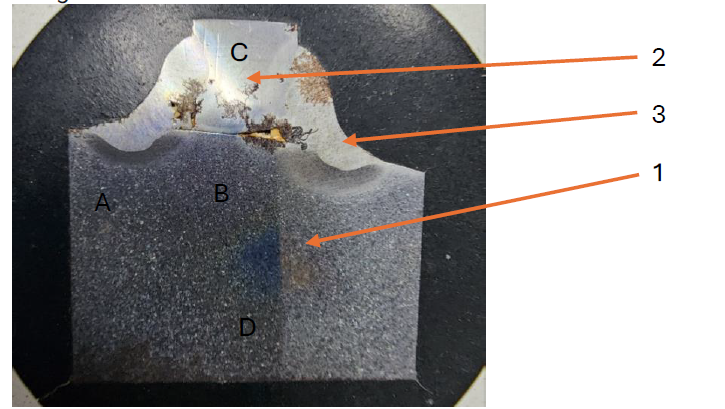
\includegraphics[width=0.5\linewidth]{figuras/imagen 1.png}
        \label{figura1}
    \end{figure}
    \item Composición química material 1:
        \begin{table}[h]
            \begin{tabular}{|l|l|l|l|l|l|l|l|}
            C\%   & Si\%  & Mn\%  & P\%   & S\%   & Cr\%  & Mo\%  & Ni\%  \\
            0,455 & 0,231 & 0,745 & 0,005 & 0,003 & 0,041 & 0,007 & 0,037
            \end{tabular}
        \end{table}
    \item Composición del material 2: acero IRAM 1020.
    \item Composición del material aporte, web: \href{https://esab.com/ar/sam_es/products-solutions/product/filler-metals/mild-steel/mig-wires-tig-rods-gmaw-gtaw/ok-autrod-12-51/}{esab-ok-autrod-12-51/}
    \item \(\textit{H}\cdot\textit{V}_0=\) obtenerla con el durómetro en la zona no tratada.
    \item \(\sigma_0=\) obtenerlo de la hoja técnica del acero que corresponda por hoja técnica.
    \item \(d=\) medirla con el microscopio.
    \item modelo físico matemático:
    \item \(\sigma_y=\) usar el modelo de Hall Petch.
    \item \(\textit{H}\cdot\textit{V}_0=\) usar el dato medido en alguno de los durómetros del laboratorio.
\end{itemize}

\section{ORIENTACIONES:}

    \subsection{ORIENTACIÓN 001: Emplear la técnica del paper de referencia:}
    \begin{itemize}
        \item Artículo científico:  Baker, B.; Menon, E.; Mcnelley, T.; Brewer, L.; El-Dasher, B.; Farmer, Joseph, C.; Torres, S.; Mahoney, M.; Sanderson, S. (2014). Processing-Microstructure Relationships in Friction Stir Welding of MA956 Oxide Dispersion Strengthened Steel. Metallurgical and Materials Transactions E. 1. 1-13. DOI: \href{http://dx.doi.org/10.1007/s40553-014-0033-6}{10.1007/s40553-014-0033-6}. Sitio Web: \href{https://www.researchgate.net/publication/305807425_Processing-Microstructure_Relationships_in_Friction_Stir_Welding_of_MA956_Oxide_Dispersion_Strengthened_Steel#fullTextFileContent}{researchgate}.
        \item Último párrafo de la Sección IV + la Figura 14:\\
        Cuando los datos de dureza actuales se trazan frente a la raíz cuadrada inversa del tamaño de grano del material de la zona de agitación, se observa una gráfica relativamente lineal para cuatro de las condiciones de FSW (Figura 14). Esta relación lineal sugiere la relación Hall-Petch que describe la conexión entre el tamaño del grano y el límite elástico en materiales cristalinos. Por el contrario, la dureza del material base es mucho mayor y no cae en esta línea de regresión lineal. Se reconoce que la dureza es una medida de la resistencia al flujo plástico de un material y, por lo tanto, es una función tanto del límite elástico como del endurecimiento por deformación. Un trabajo reciente de Baker et al. Ha realizado experimentos reales de tracción uniaxial en material extraído de la zona de agitación. El límite elástico a temperatura ambiente del material de la zona de agitación sigue, de hecho, una relación de Hall-Petch. La principal diferencia en el límite elástico a baja temperatura entre el material base y el material de la zona de agitación; por lo tanto, se debe al engrosamiento de las partículas de itrio-óxido de aluminio en el material con la correspondiente pérdida en la fuerza de dispersión. Esta pérdida de fortalecimiento por dispersión es la razón por la que el valor de dureza del material base no cae en la línea Hall-Petch de la Figura 14. Se pueden encontrar más detalles sobre la evolución de estos óxidos y su impacto en el comportamiento a tracción del material de soldadura en otros trabajos recientes. por Baker.
            \begin{figure}[h]
                \centering
                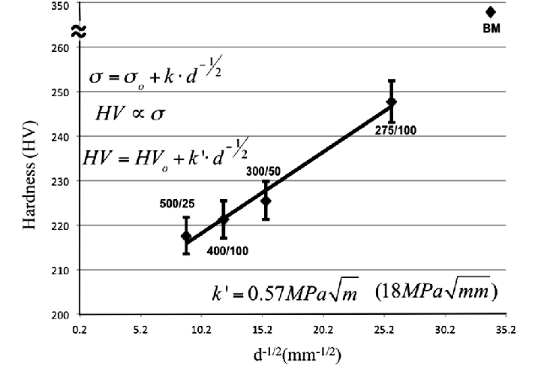
\includegraphics[width=0.5\linewidth]{figuras/imagen 2.png}
                \label{figura2}
            \end{figure}
    \end{itemize}

    \subsection{ORIENTACIÓN 002: Información de referencia.}
    \begin{itemize}
        \item Contenido de Carbono Equivalente. Sitio Web: \href{https://academia-lab.com/enciclopedia/contenido-de-carbono-equivalente/}{academia-lab}.
    \end{itemize}

    \subsection{ORIENTACIÓN 003: Información de referencia:}
    \begin{itemize}
        \item Anexo IV. Guía de métodos alternativos para determinar el precalentamiento en la soldadura de aceros estructurales. Sitio Web: \href{http://contenidos.inpres.gob.ar/docs/Reglamentos/CIRSOC-304-Reglamento.pdf}{contenidos.inpres}.
    \end{itemize}

    \subsection{ORIENTACIÓN 004: Información de referencia:}
    \begin{itemize}
        \item Emplear el modelo de referencia mencionado en el artículo científico: Sáenz, P. (1989) \textit{«Cálculo para determinar la resistencia a la tracción de algunos materiales conociendo la dureza brinell y lo inverso»}, Informador Técnico, 39, pp. 16-19. Sitio Web: \href{https://revistas.sena.edu.co/index.php/inf_tec/article/view/1250%20%E2%80%9D%20[https://revistas.sena.edu.co/index.php/inf_tec/article/view/1250/1361]}{revistas.sena}.
    \end{itemize} 

    \subsection{ORIENTACIÓN 005: Información de referencia:}
    \begin{itemize}
        \item Endurecimiento del borde de grano.  Sitio Web: \href{https://es.wikipedia.org/wiki/Endurecimiento_del_borde_de_grano}{wikipedia.org} [Figura 1: El endurecimiento de Hall-Petch está limitado por el tamaño de las luxaciones. Una vez que el tamaño de grano alcanza aproximadamente 10 nanómetros, los bordes del grano comienzan a deslizarse.].
        \begin{figure}[h]
            \centering
            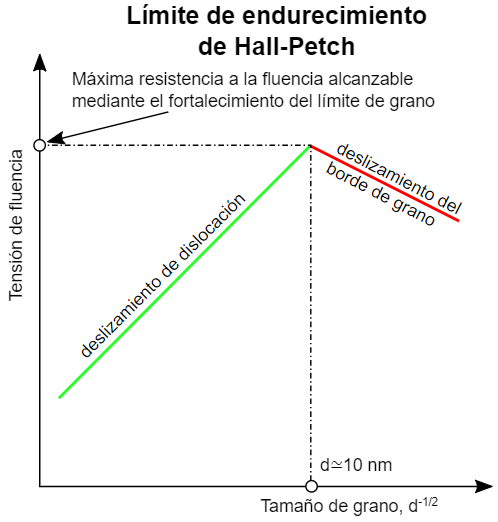
\includegraphics[width=0.5\linewidth]{figuras/imagen 3.png}
            \label{fig:enter-label}
        \end{figure}
    \end{itemize}

\section{}

\end{document}
